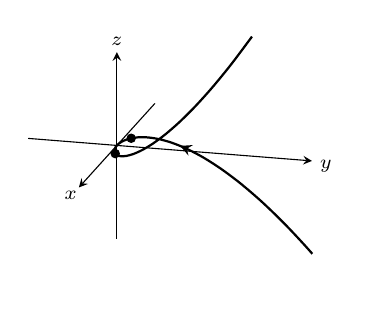
\begin{tikzpicture}[>=stealth]
\begin{axis}%
[width=175pt,tick label style={font=\scriptsize},axis on top,
			axis lines=center,
			view={105}{25},
			name=myplot,
			xtick=\empty,
			ytick=\empty,
			ztick=\empty,
			ymin=-.5,ymax=1.1,
			xmin=-.9,xmax=.9,
			zmin=-1.1, zmax=1.1,
			every axis x label/.style={at={(axis cs:\pgfkeysvalueof{/pgfplots/xmax},0,0)},xshift=-3pt,yshift=-3pt},
				xlabel={\scriptsize $x$},
			every axis y label/.style={at={(axis cs:0,\pgfkeysvalueof{/pgfplots/ymax},0)},xshift=5pt,yshift=-2pt},
				ylabel={\scriptsize $y$},
				every axis z label/.style={at={(axis cs:0,0,\pgfkeysvalueof{/pgfplots/zmax})},xshift=0pt,yshift=4pt},
				zlabel={\scriptsize $z$}
			]
%\addplot3[domain=180:270,smooth,y domain=0:90,surf,%fill=white,
%colormap={mp2}{\colormapplaneone},faceted color=black!40,samples=10,samples y=10,very thin,z buffer=sort] ({cos(y)*1.5*cos(x)},{sin(y)*cos(x)},{sin(x)});
%

\addplot3[domain=-1:1,,thick,smooth,samples y=0,{\colorone},samples=30,] ({x},{x^2},{2*x^3});

\filldraw (axis cs:-0.189, 0.035721, -0.0135025) circle (1.5pt)
					(axis cs:0.189, 0.035721, 0.0135025) circle (1.5pt);

\draw [->,thick,{\colorone}] (axis cs:-0.5, 0.25, -0.25)--(axis cs:-0.49, 0.2401, -0.235298);
%%\ifthenelse{\boolean{colorprint}}{%
%%%%%%%  Printing in color
%%\addplot3[domain=0:360,,thick,smooth,samples y=0,red,%surf,%fill=white,
%%samples=30,] ({cos(x)},{3*sin(x)},{0});
%%\addplot3[domain=0:360,,thick,smooth,samples y=0,red,%surf,%fill=white,
%%samples=30,] ({cos(x)},{0},{2*sin(x)});
%%\addplot3[domain=0:360,,thick,smooth,samples y=0,red,%surf,%fill=white,
%%samples=30,] ({0},{3*cos(x)},{2*sin(x)});
%%
%%%%% end printing in color
%%}{%
%%%%% printing in BW
%%\addplot3[domain=0:360,,thick,smooth,samples y=0,black,%surf,%fill=white,
%%samples=30,] ({cos(x)},{3*sin(x)},{0});
%%\addplot3[domain=0:360,,thick,smooth,samples y=0,black,%surf,%fill=white,
%%samples=30,] ({cos(x)},{0},{2*sin(x)});
%%\addplot3[domain=0:360,,thick,smooth,samples y=0,black,%surf,%fill=white,
%%samples=30,] ({0},{3*cos(x)},{2*sin(x)});
%%%%%% end printing BW
%%}



%\draw (axis cs:1.32,0,-.2) node (A2) {};
%\draw (axis cs:0,.8,-.3) node (B2) {};
%\draw (axis cs:-1.5,.3,-.15) node (C2) {};
%
%\draw (axis cs:.5,0,-.9) node (B2) {};


\end{axis}

%\draw (.75,.6) node [align=center](A1) {\scriptsize in plane\\[-4pt] \scriptsize $y=0$};
%\draw (3.5,.6) node [align=center](B1) {\scriptsize in plane\\[-4pt] \scriptsize $x=0$};
%\draw (3.5,3) node [align=center](C1) {\scriptsize in plane\\[-4pt] \scriptsize $z=0$};
%\draw [->] (CC) -- (B2);
%
%\draw [->](A1)--(A2);
%\draw [->](B1)--(B2);
%\draw [->](C1)--(C2);
%\draw [->](A1)--(A3);
%\draw (A1)  node[align=center,fill=white] {\scriptsize in plane\\[-4pt] \scriptsize $y=0$};


\end{tikzpicture}












